%=========================================%
%-->    Lab: Two Difference Amplifiers <--%
%--> Author: Charles Edward Pax        <--%
%-->   Date: Date 2006.03.08           <--%
%=========================================%
%
%
\documentclass[11pt,onecolumn]{article}

\usepackage{color,graphics}

\begin{document}
\title{Two Difference Amplifiers}
\date{\today}
\author{Charles Edward Pax}
\maketitle

%=====================%
%--> Sec: Abstract <--%
%=====================%
\abstract{A three op-amp instrumentation amplifier and a one op-amp difference amplifier are constructed and examined.}

%=========================%
%--> Sec: Introduction <--%
%=========================%
\section{Introduction}\label{sec:Introduction}
The instrumentation amplifier has been discussed in class and in the Faissler textbook. The circuits built in this lab are somewhat complicated and it was necessary to take care in organizing the design, such as color coding, for example. A 10K potentiometers were used to adjust each opamp to a gain of 1.

%============================%
%--> Sec: Data & Analysis <--%
%============================%
\section{Data \& Analysis}\label{sec:DataAndAnalysis}
\subsection{Difference Amplifier}
The bridge circuit in Figure \ref{fig:Diagram1} was constructed in order to supply $V_1$ and $V_2$ to the amplifier circuit by setting $RB_1 = RB_2 = RB_3 \approx 3$ k$\Omega$ and $RB_4 = 5$ k$\Omega$ potentiometer in series with a 1 k$\Omega$ resistor. The voltage at the center terminals of the bridge were found to be $\approx 5.98$ V. The difference amplifier shown in Figure \ref{fig:Diagram2} was constructed such that $R_1 = R_2 = 10$ k$\Omega$ and $R_3 = R_4$\footnote{Should I have a value for $R_3$ and $R_4$?} to give a gain of 10.
%
% Figure: Diagram1
%
\begin{figure}
\center
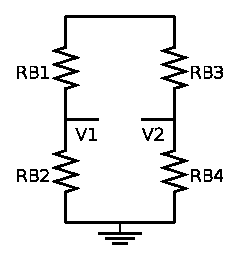
\includegraphics{Diagram1.eps}
\caption{Bridge circuit.}\label{fig:Diagram1}
\end{figure}
%
% Figure: Diagram2
%
\begin{figure}
\center
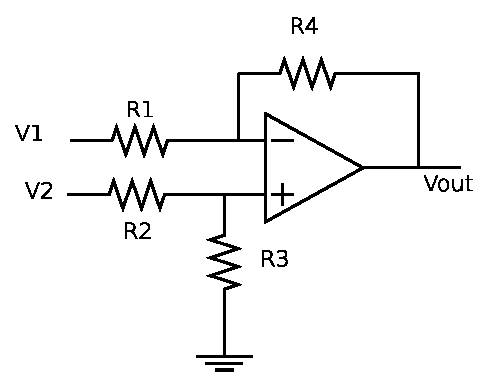
\includegraphics{Diagram2.eps}
\caption{Difference amplifier.}\label{fig:Diagram2}
\end{figure}

The potentiometer was adjusted to $V_1 - V_2 = 0$ by measuring the voltage difference with a voltmeter. The op-amp circuit in Figure \ref{fig:Diagram2} was connected to the bridge circuit in Figure \ref{fig:Diagram1}. There was an offset of \_\_\_\_\_\_ measured\footnote{What was the offset measured?} and was subtracted from subsequent measurements.

$V_1 - V_2$ was varried to measure the output voltage versus $V_1 - V_2$ for about six voltages between -0.8 and 0.8 V. The linear relationship of $V_{out}$ and $V_1 - V_2$ is easily observable in Figure \ref{fig:Plot01}
%
% Figure: Plot1
%
\begin{figure}
\center
\input{Plot01}
\caption{Relationship of $V_{out}$ as a function of $V_1 - V_2$ in the bridge circuit-amplifier combination. A plot of $V_{out}$ with $V_1$ and $V_2$ beging varried directly is also plotted.}\label{fig:Plot01}
\end{figure}

$V_1$ and $V_2$ were then disconnected from the bridge circuit. $V_2 = 0$ was set and voltages for $V_1$ were varried between -0.8 and 0.8. The resulting measurements are also plotted in Figure \ref{fig:Plot01}. As can be seen from the graph, this relationship is also linear, but inversly so.

With $V_2 = 0$ a sine wave was input with a maximum amplitude of 0.5 V. The gain depends on the frequency such that\footnote{Finish this statement.}. The gain = 0 at approximatly 262 kHz.

\subsection{Instrumentation Amplifier}
The Instrumentation amplifier is the circuit shown in Figure \ref{fig:Diagram3}. The gain for which is
%
% Equation: GainIA
%
\begin{equation}\label{eq:GainIA}
\frac{V_{out}}{\left( V_1 - V_2 \right)} = -k\left( 1 + 2a \right)
\end{equation}
with the first stage having a gain of $1 + 2a$ and the second stage having a gain of $k$. The circuit was constructed such the gain is $\approx 10$ by setting $R_1 = 100$ k$\Omega$, $R_2 = 10$ k$\Omega$, $R_1/a = 10$ k$\Omega$, $a = 10$.
%
% Figure: Diagram3
%
\begin{figure}
\center
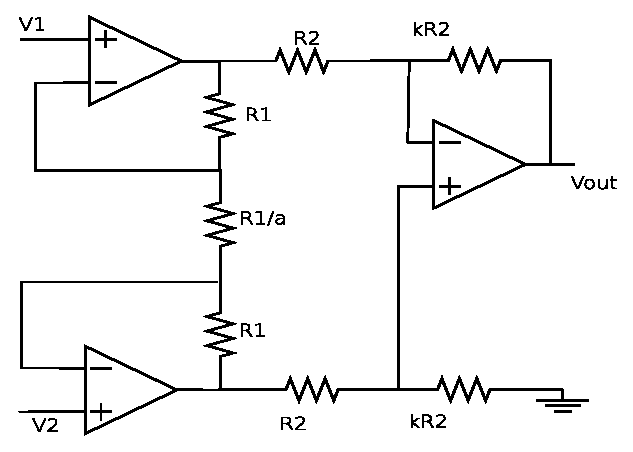
\includegraphics{Diagram3.eps}
\caption{Instrumentation Amplifier.}\label{fig:Diagram3}
\end{figure}


%=======================%
%--> Sec: Discussion <--%
%=======================%
\section{Discussion}\label{sec:Discussion}

\end{document}
